
\chapter{Model}\label{ch:model}

The goal of the model is to transform a sequence of spectral input features $x^{(i)}$
into a transcript sequence $y^{(i)}$.
In fact, the model for each time step $t$ in sequence $x^{(i)}$ estimates the probability
distributions $\mathbb{P}(\ell | x^{(i)}_t)$ over each letter $\ell$ in the alphabet.
Then, the sequence of probability distributions is decoded using the \textit{CTC Inference} algorithm,
which returns the most probable transcript $\hat{y}^{(i)}$.
Additionally, one can extend a decoding process and use the \textit{External~Language~Model}
either the char or the word-based, which helps to correct minor language mistakes.

The model solves two closely related tasks.
It learns to recognize phonemes and formulate grammar rules at the same time.
Conceptually, the model can be divided into two sub-models \textit{Phoneme Model},
and \textit{Implicit~Language~Model}, where a boundary between them is fuzzy.
In fact, a model is able to parallel and accurate build both of them, when a training corpus is large enough.
However, inflected languages such as~Polish contains much more
grammar rules to define than in the case of English.
In Polish, there are complex grammar rules such as~('ó/u',~'ż/rz'~or~'t/d'), silent letters,
and numerous prefixes and suffixes.
Therefore, in order to achieve comparable results in the Polish language, the corpus must
be substantially larger than the one presented for the English language~\cite{amodei2015}.

In our case, the Polish language is complex, the training corpus is small and the transcriptions
are duplicated (Chapter~\nameref{ch:data}), that's why the \textit{Implicit~Language~Model} is imprecise.
The inflection of the Polish language and the imprecise model yield the mistakes with a large
\textit{char~edit~distance}, that are hard to decode, in particular using external static
language models (either the char or word-based \textit{n-gram models}).
A dedicated, separate, and more sophisticated external language model can be created,
and as a decoder can try to correct mistakes.
However, still, the decoder can not solve complex problems, because it operates on
sparse probability distributions returned by the model.

In this chapter we present two models the \textit{Base~Model} and the \textit{Synthetic~Boosted~Model}.
The base model is a recurrent neural network with the objective \textit{CTC~Loss} (Chapter~\nameref{ch:background}).
Whereas the \textit{Synthetic~Boosted~Model} is an extension of the base model with the built-in
decoder \textit{Synthetic~Language~Model}, which, thanks to the synthetic data, increases
the amount of language information supplied to the model.
The \textit{Synthetic~Language~Model} is able to solve complex problems because
it operates on hidden states $h$ of the base model, which are rich in information.


\section{Base Model}\label{sec:base-model}
The base model architecture is built upon the \textit{Deep~Speech~2} model, which is
the continuation of the \textit{Deep~Speech} success~\cite{hannun2014,amodei2015}.
The model contains a convolutional layer and then several recurrent layers (figure~\ref{fig:base_model}).
At the end of the model, there is an output layer that, for each time step $t$ in the input sequence $x^{(i)}$,
returns the probability distributions $\mathbb{P}(\ell | x^{(i)}_t)$ over each letter $\ell$ in the alphabet.

\begin{figure}[!h]
    \centering
    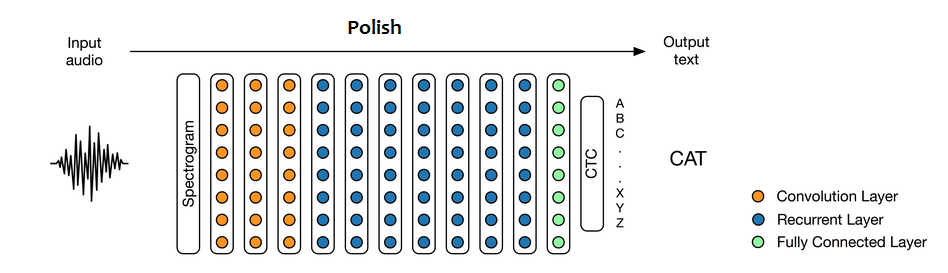
\includegraphics[width=12cm]{figures/base_model.png}
    \caption{
The architecture of the Base Model.
The figure is adopted from~\cite{ryan2016}.
}
\label{fig:base_model}
\end{figure}

\subsection*{Convolutional Layer}

The first layer of the \textit{Base~Model} is a two-dimensional (\textit{time-and-frequency domain}) convolutional layer.
The layer analyses a small context bounded by a \textit{receptive field} with size in frequency $c_f$ and time $c_t$.
The layer representation is defined by $h^{l}$, assuming that $h^{0}$ represents input data $x$.
Convolutional layer activations can be written for the $i$-th activation at time $t$ and frequency $f$ as:
\begin{equation}
h^{l}_{t,f,i} = \mathcal{F}(w^{l}_i * h^{l-1}_{t-ct,t+ct:f-cf,f+cf})
\end{equation}
where $*$ means a convolve of the $i$-th filter with the receptive field of the input data,
and $\mathcal{F}(\cdot)$ is an unary, non-linear function.
We have selected the \textit{Clipped Rectified-linear} (ReLU) $\sigma(x) = \min\{\max\{x, 0\}, 20\}$,
as an activation function.
We used the \textit{same} convolution to keep constant the number of features in both frequency and time.\footnote{
The activation function is limited to avoid exploding of the gradient (in particular the first phase of training).
}

For a long time, \acrshort{asr} systems used \textit{Temporal Convolution}, which is a one-dimensional
convolutional layer (along the time dimension).
It analyzes the small context of a signal,
which is composed of concatenation of previous and subsequent $C$ input feature vectors~\cite{dahl2011,ghoshal2013,hannun2014}.
However, the two-dimensional convolutional layer more precisely reflects the audio \textit{spectral variance}
by sharing filter weights also in the frequency domain.
In consequence, the two-dimensional convolutional layer reduces the number of parameters, is resistant to shifts
in frequency ranges, and significantly accelerates optimization, when the \textit{stride} is applied.
Therefore the two-dimensional convolutional layer is often used in ASR systems~\cite{abdel-hamid2012,sainath2013,soltau2014}.

\subsection*{Recurrent Layers}

The next layers of the \textit{Base~Model} are the bidirectional recurrent layers,
which constitute the core of the model, because they contain more than 95\% of network parameters.
Either the \textit{fully connected} layer or the \textit{convolutional} layer builds the $h^l_t$ representation
exclusively based on the preceding representation $h^{l-1}_t$.
The recurrent layer is unique because it also has the loop $h_{t-1}$ which in fact gives a view to all previous steps.
In consequence, a representation $h^l_t$ is built upon the broad backward context.

Moreover, the bidirectional recurrent layer exists, which has at time $t$ both the backward context $h_{t-1}$,
and the forward context $h_{t+1}$.
The forward $\overrightarrow{h}^l$ and backward $\overleftarrow{h}^l$ layer activations at time $t$ are defined as:
\begin{align}
\overrightarrow{h}^l_t = \mathcal{F}(h^{l-1}_t, \overrightarrow{h}^l_{t-1}) \\
\overleftarrow{h}^l_t = \mathcal{F}(h^{l-1}_t, \overleftarrow{h}^l_{t+1})
\end{align}
Then the components are summed, and the bidirectional recurrent layer activation is
equal to $h^l_t=\overrightarrow{h}^l_t + \overleftarrow{h}^l_t$.
There are many different variants of the function $\mathcal{F}(\cdot)$, which
works successfully in the \acrshort{asr}.
In the base model, we selected the widely used \textit{Long Short-Term Memory} (\acrshort{lstm})
layer~\cite{hochreiter1997} (and explained in~\cite{olah2015}),
which can discover long dependencies and has publicly available highly efficient implementation.

The \acrshort{lstm} layer, in relation to a vanilla \acrshort{rnn} presented in the~Chapter~\nameref{ch:background},
has in addition the cell state, the vector $C_t$, which describes the \textit{general} context at time $t$.
The cell state is modified by two gates the \textit{Forget gate layer} $f_t$ and
the \textit{Input gate layer} $i_t$ based on vectors $h^{l-1}_t$ and $h^l_{t-1}$:
\begin{align}
&f_t = \sigma(\mathbb{W}^{(f)} \cdot [h^{l-1}_t, h^l_{t-1}] + b^{(f)}) \\
&i_t = \sigma(\mathbb{W}^{(i)} \cdot [h^{l-1}_t, h^l_{t-1}] + b^{(i)}) \\
&\tilde{C_t} = \tanh(\mathbb{W}^{(C)} \cdot [h^{l-1}_t, h^l_{t-1}] + b^{(C)}) \\ \label{eq:tanh}
&C_t = f_t \circ C_{t-1} + t_t \circ \tilde{C_t} \label{eq:lstm_state_update}
\end{align}
where $\circ$ means a pointwise multiplication.
The \textit{Forget Gate Layer} decides which features to erase in the general context $C_{t-1}$.
The \textit{tanh} gate creates the group of potential candidates for new features $\tilde{C_t}$, and
the \textit{Input Gate Layer} defines how important they are in the general context $C_t$.
At the end, there is the \textit{Output Gate Layer}, which returns the representation $h^l_t$
by the view of the current cell state $C_t$ via the filter $o_t$:
\begin{align}
&o_t = \sigma(\mathbb{W}^{(o)} \cdot [h^{l-1}_t, h^l_{t-1}] + b^{(o)}) \\
&h_t = o_t \circ \tanh{C_t}
\end{align}

The recurrent layers are the essential elements of the model.
Thanks to the recurrent layers, a model based on the large training dataset,
can build the rich \textit{Implicit~Language~Model}.

\subsection*{Output Layer}
At the end of the model, there is a linear layer with the activation function~\textit{softmax},
which returns, for each time step $t$ in the input sequence $x^{(i)}$,
the probability distribution of occurrence of each character from the alphabet $\ell$ at time $t$:

\begin{equation}
    \mathbb{P}(\ell_t = k | x) = \frac{\exp(w_k^L \cdot h_t^{L-1})}{\sum_{j}\exp(w_j^L \cdot h_t^{L-1})}
\end{equation}


\section{Synthetic Boosted Model}\label{sec:synthetic-boosted-model}

The \textit{Synthetic~Boosted~Model} is composed of two integrated parts, the \textit{Phoneme~Model}
and the \textit{Synthetic~Language~Model}, which are optimized in the separated trainings
(figure~\ref{fig:synthetic_boosted_model}).
The \textit{Synthetic~Boosted~Model} formulates the grammar rules using a much larger,
synthetically augmented training corpus.
The model for the input sequence $x^{(i)}$ returns, as the base model does, the sequence of probability
distributions $\mathbb{P}(\ell | x^{(i)}_t)$ over each letter $\ell$ in the alphabet for each time step $t$.

\begin{figure}[!h]
    \centering
    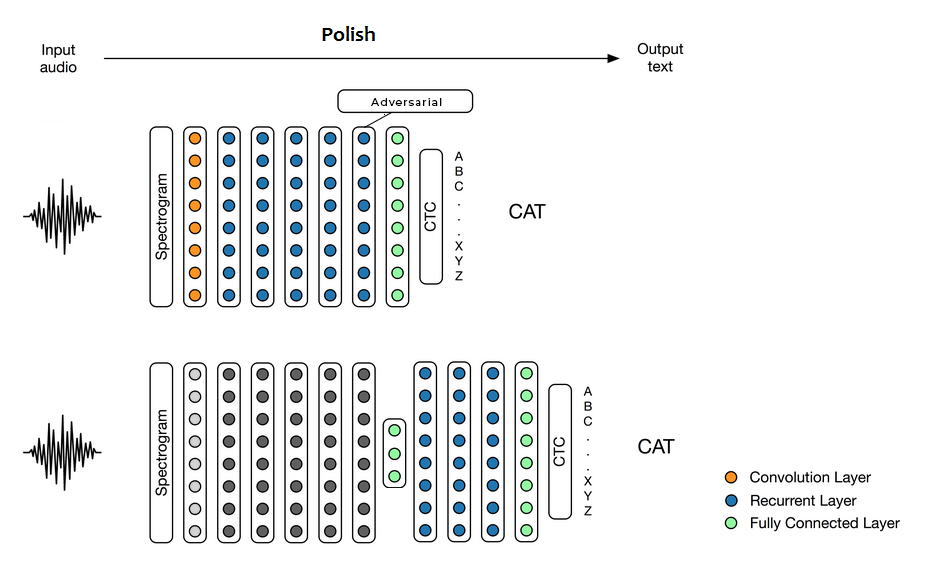
\includegraphics[width=12cm]{figures/synthetic_boosted_model.png}
    \caption{
The architecture of the Synthetic Boosted Model.
The figure is adopted from~\cite{ryan2016}.
}
\label{fig:synthetic_boosted_model}
\end{figure}

The use of a synthetic data up to the ration 1 to 1, an authentic to a synthetic data,
is a widely practiced technique of augmentation the training dataset.
Naively adding more synthetic data to a training dataset brings a decline in performance.
The authentic samples are overwhelmed by the synthetic ones, what in consequence,
reduces the ability of actual phoneme recognition.
Therefore, training is divided into two stages.
Firstly, we train the \textit{Phoneme~Model} (upper figure~\ref{fig:synthetic_boosted_model})
on a dataset with the ratio 1 to 1, an authentic to a synthetic data.
Then, we train the \textit{Synthetic~Language~Model} (lower figure~\ref{fig:synthetic_boosted_model}),
which processes several times larger synthetically augmented training corpus.
The \textit{Phoneme~Model} is frozen (weights are not updated) to protect the ability
of actual phoneme recognition, therefore it plays a feature extractor role exclusively at this stage.
Finally, the purpose of the \textit{Synthetic~Language~Model} is to \textit{boost}
the representation $h$ created by the frozen \textit{Phoneme~Model}, and return
the correct prediction.


\subsection*{Phoneme Model}

The \textit{Phoneme~Model}, like the base model, is made up of the convolutional layer,
and then from several recurrent layers.
It also has an output~layer, which is removed after training.
The model is optimized with the ratio 1 to 1, an authentic to a synthetic data,
with the modified loss function.

The aim is to build the accurate \textit{Phoneme~Model}, which also produces
the independent of data source representations~$h$, the last \acrshort{lstm} hidden states.
For easily distinguishable representations, the \textit{Synthetic~Language~Model} constructs
separate rules for authentic and synthetic data, which is an undesirable phenomenon.
To achieve more independent representations, we add the \textit{adversarial} component to the loss function.
We propose the simple function that measures in every \textit{mini-batch} the average activation vectors
for both authentic $\mathbf{\bar{h}}_{a}$ and synthetic samples $\mathbf{\bar{h}}_{s}$, and then
calculates their \textit{Manhattan} distance:
\begin{equation}
\mathcal{L}_{Adv} = \|\mathbf{\bar{h}}_{a} - \mathbf{\bar{h}}_{s} \|_{1}
\end{equation}
In consequence, the loss function has two components the \textit{CTC Loss} and the \textit{Adversarial Loss},
and is defined as the weighted sum:
\begin{equation}
\mathcal{L} = w_0 \cdot \mathcal{L}_{CTC} + w_1 \cdot \mathcal{L}_{Adv}
\end{equation}
where in every single \textit{mini-batch} we provide an equal number of authentic and synthetic samples.


\subsection*{Synthetic Language Model}

The \textit{Synthetic~Language~Model} is made up of the narrow \textit{fully-connected} layer
(called the \textit{projection}), and then several recurrent layers, and an \textit{output~Layer},
which are the same as in the base model.
Despite the modified loss function imposed on the \textit{Phoneme~Model}, representations $h$ are
still highly dependent on the source of data.
Therefore, we introduce the \textit{projection} layer, which forces to reduce the number of dimensions.
Thanks to dimension reduction, the representations are more independent of the data source,
but much of the information is lost.

The \textit{Phoneme~Model} seamlessly learns to correctly recognize synthetic data.
The aim is to build the training process, where the \textit{Phoneme~Model} makes
\textit{similar} mistakes on synthetic data as on authentic data.
For this purpose, we mask randomly selected parts of the spectrogram (Chapter~\nameref{ch:data}).
In this way, we simulate the situation in which the \textit{Phoneme~Model} has difficulty to recognize
the phoneme on authentic data, and the \textit{Synthetic Language Model} tries to correct it.
The process is analogous to an unsupervised language modeling on raw text.
Based on the context, the model tries to estimate the masked part of the input.
In consequence, we can learn language dependencies processing masked synthetic data.
